
% It is an example which *does* use the .bib file (from which the .bbl file
% is produced).
% REMEMBER HOWEVER: After having produced the .bbl file,
% and prior to final submission,
% you need to 'insert'  your .bbl file into your source .tex file so as to provide
% ONE 'self-contained' source file.
% For tracking purposes - this is V3.1SP - APRIL 2009

\documentclass{acm_proc_article-sp}
%\documentclass{sig-alternate}

\usepackage[hyphens]{url}
\usepackage{graphicx}
\usepackage{eurosym}
\usepackage{stfloats}
%\usepackage[breaklinks,colorlinks=true,linkcolor=black,urlcolor=black,citecolor=black]{hyperref}

\makeatletter
\def\@copyrightspace{\relax}
\makeatother

\widowpenalty=1000
\clubpenalty=1000

\begin{document}

\title{Computer Secondary Storage}
\subtitle{Seminar: Use of Modern Hardware in Big Data Processing}

\numberofauthors{1}
\author{
\alignauthor
Sascha K{\"o}nigsberg, Claus Strasburger\\
       \affaddr{Technische Universit{\"a}t M{\"u}nchen}\\
       \email{\texttt{\{sascha.koenigsberg, c.strasburger\}@tum.de}}
}

\date{20 May 2014}

\maketitle
\begin{abstract}
This report contains a summary of developments in computer secondary storage, particularly in big data server environments. It describes the history of \emph{Hard Drives} and \emph{Solid State Disks} and list tradeoffs and considerations of the currently available options. It further presents the concept of \emph{Phase Change Memory}, a possible alternative for the future of secondary storage, its history and current state of research. It provides a summary of the presented techniques and trends.%% fazit?
\end{abstract}

\category{B.3.2}{Memory Structures}{Design Styles}[mass storage, primary memory]
\category{D.4.2}{Operating Systems}{Storage Management}[secondary storage, storage hierarchies]

\terms{Management, Performance, Reliability}

\section{Introduction}
When we talk about computer secondary storage, we should briefly explain what secondary storage is. As the name suggests there also exists primary storage in computers. The latter part of the memory hierarchy contains the CPU registers, CPU caches (cache levels one to three) and the main memory (\emph{DRAM}). Main memory is directly accessible by the CPU and volatile, e.g. stored data is not preserved on power loss. This means that all data are lost if the power supply is interrupted or the computer is shut down. Computer secondary storage is in the memory hierarchy one layer below the RAM. It includes flash memory (like SSD, USB flash drives), optical discs (CD-ROM, DVD), magnetic discs (HDD, Floppy) and magnetic tape (Compact Cassette). Secondary storage is also known as external memory and differs from primary storage in that it is not directly accessible by the CPU. The computer usually uses its input/output channels to access secondary storage. It is non-volatile --- it keeps data on power loss. In this report, we focus on hard disk drives and solid state drives.
\\
Hard disk drives, as schematized in Figure~\ref{fig:hdd}, use magnetic coated rotating disks (called \emph{platters}) to store data. The direction of magnetization represents binary data bits. The actuator head detects and modifies the magnetization. The actuator arm moves to the correct cylinder on the disc and waits for the platter to rotate until the data is below the actuator head.


\begin{figure}[ht]
\centering
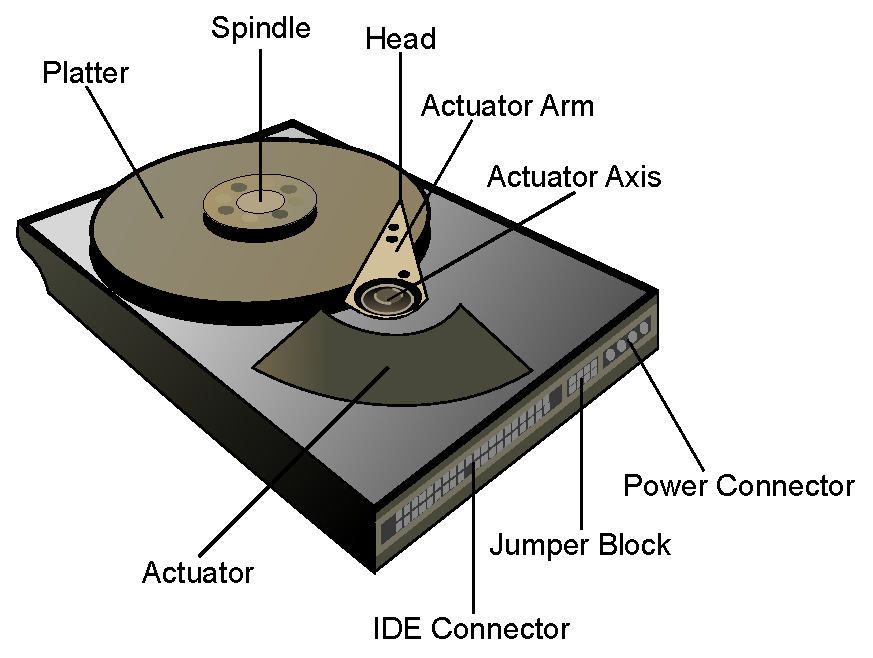
\epsfig{file=hdd-en.eps, width=\columnwidth}
%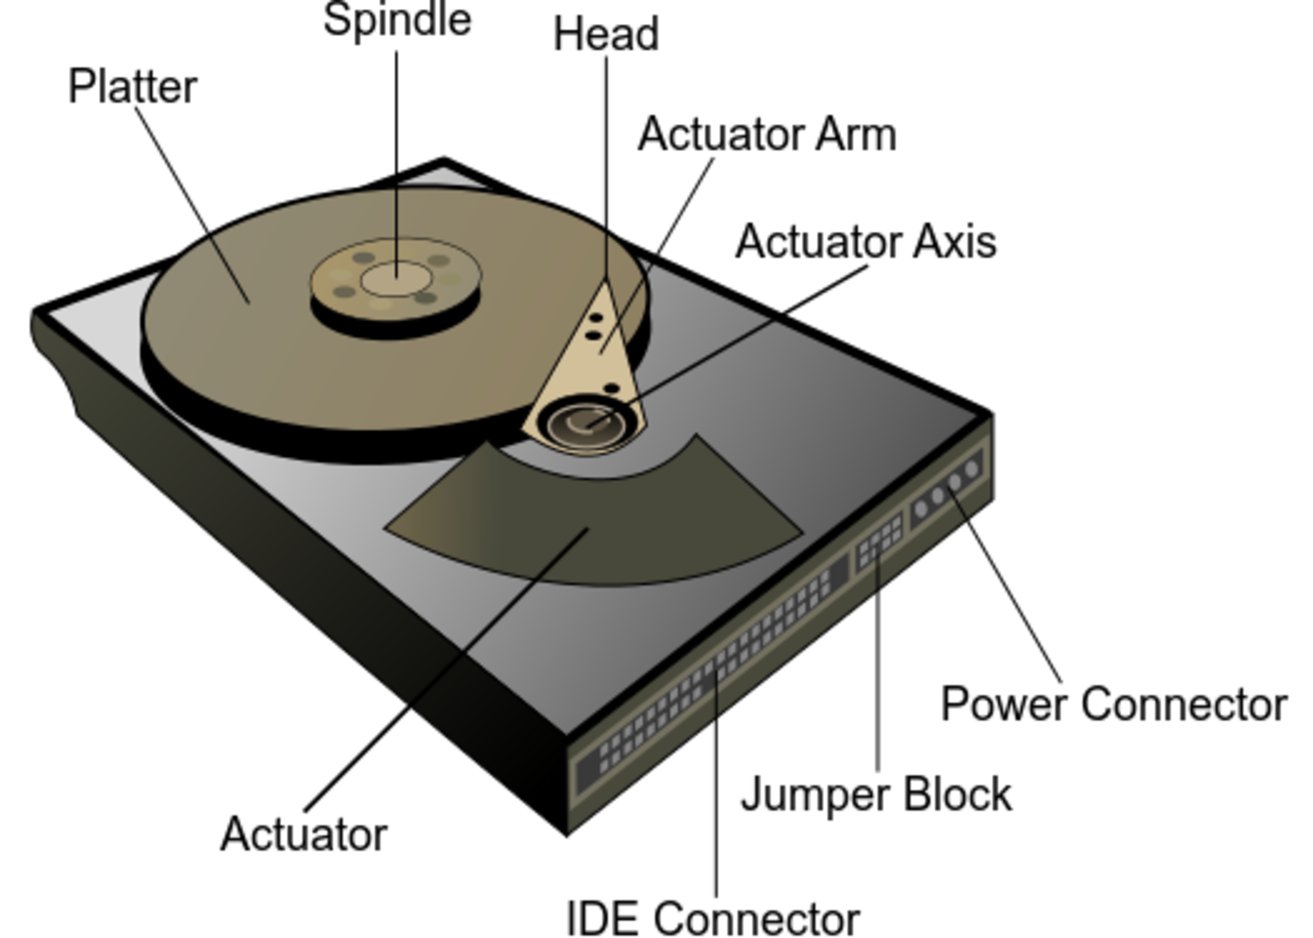
\includegraphics[width=\columnwidth]{hdd-en.png}
\caption{Hard Disk schematic~\cite{wikihdd}}
\label{fig:hdd}
\end{figure}
Solid state drives use two key components: The controller and the memory. The controller is an embedded processor and connects the host computer with the memory. It executes code on firmware-level and performs many functions necessary for SSD operation. These include generating an Error-correction code (ECC), Wear-leveling, garbage collection and encryption.
\\
The controller is important for the performance of a SSD. For example, if the controller provides multiple channels and can address them all in parallel, multiple input/output operations can happen simultaneously on different memory chips, which increases the speed and response time dramatically. The memory is of course the location where data are saved on and usually consists of NAND flash, DRAM or a combination of both. NAND is cheaper and non-volatile but is slower than DRAM. Most SSDs are used as long-time storages requiring non-volatile memory, which means that most SSDs use NAND flash memory. These memory chips can be organized as Single-level cell (\emph{SLC}) or Multi-level cell (\emph{MLC}). SLC is ten times more persistent and allows three times faster sequential write, with nearly the same sequential read performance, but it is 30\% more expensive. The usage of SLC or MLC chips is mostly determined by pricing: Cheap SSDs use MLC chips, while high performance enterprise SSDs use SLC.
\\
\begin{table*}[bh]
\centering
\caption{Comparison of SSDs and HDDs}
\label{table:comparison}
\begin{tabular}{r|cc}
									& SSD						& HDD				\\ \hline \hline
Power consumption: idle / access		& 0.1 / 5.8 W				& >4 / >6 W			\\ \hline
Access time: Read / Write 			& 0.2 / 0.4 ms				& >3.5 / >3.5 ms	\\ \hline
Data transfer rate: Read / Write		& >500/ >500 MB/s			& <160 / <160 MB/s	\\ \hline
Mechanical properties / mobility		& very good					& acceptable		\\ \hline
Capacity							& up to 2 TB				& up to 6 TB		\\ \hline
Write cycles (lifetime)				& 3,000 -- 100,000			& 10 Billion		\\ \hline
Price								& 500 -- 1000 \euro/TB		& 30 -- 50 \euro/TB	\\
\end{tabular}
\end{table*}
\section{History of storage drives}
\subsection{Hard Disk Drives}
Hard disk drives are the successor to drum memory. The first HDD was the IBM 350. It had a capacity of 5 MB and was as big as a locker, because the actuator arm was moved electro-pneumatically. It was announced in 1956 and was not sold but rented for 650 dollar a month. Years later, IBM started the Winchester project with the goal to develop a rotating memory with firmly mounted medium. The first HDD of the Winchester project was the IBM 3340 in 1979. The first Winchester drive in 5.25" form factor was the Seagate ST506 (in 1980). This name also became the name of the interface used by the ST506. The ST506-interface established as de-facto-standard.
%% Kommentar von meinem Vater: "Ich hatte auch einen Winchester drive. Das war ein Knüller!" hrhr
\\
In 1986, SCSI was specified, one of the first official HDD protocols. Three years later came ATA, another HDD interface. In 1997, the Giant Magnetoresistive Effect (\emph{GMR}) was first used. This is a physical effect that appears within structures with alternately magnetic and non-magnetic layers and allowed to considerably increase the storage capacity.
\\
The first Serial-ATA HDD used Native Command Queueing (\emph{NCQ}) in 2004. NCQ is a technology to reorder the input/output operations and improve performance. The first prototype of 2.5" Hybrid-HDD (\emph{H-HDD}) included NAND flash memory and was announced in 2005. The flash memory was used as cache to enhance the speed and the response time of the HDD. The 1 terabyte limit was reached by Hitachi in 2007, the 2 TB and 3 TB limit by Western Digital in 2009/2010. Important form factors of HDD are 5.25.", 3.5", 2.5" (used in laptops) and 1.8" (also used in laptops and some mobile media players, such as the Apple iPod). Important internal interfaces are ATA (IDE), ESDI, SCSI, S-ATA, Serial Attached SCSI (\emph{SAS}) and ST506 (important external interfaces: FireWire, USB and eSATA).
\\
While there were multiple manufacturers on the HDD market for years, today only Seagate, Toshiba and Western Digital produce HDDs.

\subsection{Solid State Disks}
The origins of SSDs used magnetic core memory and card capacitor read-only store (CCROS)~\cite{originssds}. They were built in the 1950s. In the 1970s and 1980s, SSDs were used in supercomputers only. The first flash-based SSD were developed by MSystems in 1995, but they were so expensive that they were only used for military applications and other less price-sensitive sectors. In 1999, BiTMICRO announced the first SSD in the 3.5" form factor. The first SSD for laptops in 2.5" and 1.8" form factors were developed by Samsung in 2006 and were sold for about 600 US-dollar. This was only an eighth of the price of previous SSDs. Although that did not yet mean the breakthrough for SSDs, Samsung could gain 45\% of market share with these models. Only one year later, Fusion-io announced the first PCIe-based SSD which reached 100,000 IOPS (as comparison: current HDDs reach up to 125 IOPS). The second generation of SSDs for consumers were the first generation that used MLC instead of SLC flash memory chips. As we have seen, this decreased the price for SSDs, but the performance was lower than SLC-based SSDs performance. In 2009, SSDs used improved MLC flash memory chips which had even better performance than some SLC chips. The term \emph{Enterprise flash drives} (\emph{EFD}) was introduced in 2008, but it became never a standard, so every SSD-manufacturer use the name EFD for their SSDs~\cite{efds}.

{\tolerance=900
\section{Advantages and disadvantages of Solid State Disks compared to Hard Disks}
}
As displayed in Table~\ref{table:comparison}, SSDs have very low access time, high data transfer rate and high number of I/O operations per second (\emph{IOPS}). Because there are no moving parts, an SSD is completely silent and very robust. This includes properties like shock resistance, temperature tolerance, dimensions, weight, etc. and leads to a very good usability in mobile computers and more reliability in a server environment, since rack mounts are prone to vibration. As we have seen when talking about SSD controllers, the speed can increase with a higher rate of parallelizability. The speed of SSDs can be so high that even the newest and most advanced interfaces for SSDs and HDDs are too slow. So modern SSDs use interfaces like \emph{mSATA}, \emph{PCI-Express} and \emph{FibreChannel}. Because of the small dimensions new form factory like \emph{mSATA}, \emph{PCIe Mini Card} and \emph{M.2} were developed too.
\\
But there are also some negative points about SSDs. SSDs are expensive; especially in terms of price per TB, when compared to HDDs. Another problem is the limited time of write cycles for every NAND-cell. We will later show the disadvantages of write amplification and its complex countermeasures.

\section{SSD challenges}
Solid State Drives pose many difficult challenges to both their manufacturers and users. Despite the superior theoretical access time and read/write bandwidth of NAND flash, the inherent limitations of NAND flash memory make development and use of SSD difficult and completely different to regular hard disk drives.
\\
\\
\subsection{Hardware Limits}
NAND flash has two major limits: Block erasure and write cycles (\emph{Memory wear}). Other limitations include Bit Corruption and Read Disturb.

\subsubsection*{Block Erasure}
Because of the higher current which is necessary to release the trapped charge in a flash memory cell compared to charging a cell, deleting information is done in blocks of cells, called \emph{Erase Blocks}. Most current Solid State Disks use blocks of 256 pages or more~\cite{codecapsule2014coding}.
This means that to write to a page which was previously written and subsequently marked as unused, either all pages on the same erase block have to be marked unused also, or pages that are currently in use have to be copied to another block. It is not until this has been done that the block can be erased. This process is called \emph{Garbage Collection}.

\subsubsection*{Limited Write Cycles}
When writing to a flash cell, charge is captured in it, similar to a capacitor.
However, when erasing it, not all charge is released. Some electrons get trapped in the gate, building up charge until the potential of an uncharged cell is indistinguishable from that of a charged cell. This phenomenon is known as \emph{Memory wear} occurs earlier in multi level cells than in single level cells, since the voltage differences between levels are smaller and the cell is unusable as soon as the trapped charge approaches the difference between two levels.
Current SLC NAND flash cell lifetimes range from hundreds of thousands program/erase (\emph{P/E}) cycles to one million before becoming useless, while multi level or triple level cells have three thousand to ten thousand cycles.

\subsubsection*{Bit Corruption}
Because of charge leaking in and out of storage cells, raw flash memory is prone to random bit errors. Error correcting codes (\emph{ECC}), as well as error detecting codes (such as Cyclic Redundancy Check, \emph{CRC}), are used to find and possibly correct errors without silently corrupting data.

\subsubsection*{Read Disturb}
Another phenomenon in NAND flash is called \emph{Read Disturb}. When a cell is accessed many times without being erased, trapped charge can build up in nearby cells, causing them to flip their status if they were uncharged before.
This happens after about one million reads without erase in single level cells and after 100 thousand reads for multi level cells~\cite{cooke2007inconvenient}.
\\
To prevent read disturb from corrupting data, SSD controllers keep count of how many times a page was read since the last erase cycle. When a predefined critical read limit is approached, the data is moved or re-programmed. Read disturb happening in spite of this prevention are handled by ECC.

\subsection{Controller Firmware Challenges}
SSD controllers have to do extensive bookkeeping to prevent the underlying flash memory from corrupting data or deteriorating. Errors or oversights in controller firmware programming can lead to drastically reduced performance, data loss or silent data corruption.

\subsubsection*{Garbage Collection}
To write data to flash memory, free pages have to be available. SSD controllers use Over-Provisioning (\emph{OP}) to keep the number of unwritten pages high during burst writes, but if more data is to be written than free pages are available, or when invalidated pages need to be reclaimed, garbage collection is necessary. In this process the controller copies still-valid pages out of blocks containing many invalid pages; only after that the whole block can be erased. As the number of invalidated or free pages decreases --- to the operating system these are known as \emph{free} space --- more garbage collection and copying of pages in use has to be done in order to ensure available pages on write requests.

\subsubsection*{Wear Leveling}
Flash cells degrade when being written. When one section of the disk is written many times, e.g. a swap file or a simple counter, the page containing that section can wear out rather quickly --- limiting the amount of overprovisioning or, in worse cases, reducing the effective size of the disk before it is at the end of its life. To prevent this from happening the controller keeps count on page writes and re-maps heavily written pages to other pages regularly.

\subsubsection*{Write Amplification}
Summing up these techniques used by the controller, write accesses to the device can lead to more data being written than requested by the operating system. These techniques include garbage collection, wear leveling, and, most prominent, small and/or f writes.
Also, in the case of read disturb mitigation, even read accesses can cause writes to the disks.
In optimal situations write amplification can be a factor of as low as $1.1\times$, while in worst-case conditions it can go up to $10\times$ or $20\times$.
\\
Some manufacturers decrease this benchmark value by compressing and deduplicating data on-the-fly before writing it to disk, but this will only show effects for compressible data and only increase overhead for data not easily compressible.

\subsection{Software Challenges}
Even though SSD manufacturers go to great lengths to ensure optimal performance and data integrity, system architects and developers still need to take specific precautions when building software or systems using SSDs. Blindly following current usage patterns established for rotating media will lead to bad performance --- possibly lower than with hard drives --- and sudden performance drop or high device failure rate.

\subsubsection*{Random Writes}
Even though SSDs have no mechanical parts, sequential writes will still be faster than small writes. Applications have to be careful to try and write in as big blocks as possible, since the smallest written unit will always be the page size (currently 8 to 16 KiB). Small random writes, such as those produced by a conventional Relational Database Management System (\emph{RDBMS}) like PostgreSQL or MySQL, will cause rapid allocation of many pages, which then need to be garbage collected. As soon as the SSD controller runs out of overprovisioned pages, garbage collection will be necessary and drastically slow down the device. The effective write amplification will be very high (depending on the write sizes and their ratio to the page and block sizes), also leading to faster memory degradation and therefore a high disk failure rate.

\subsubsection*{TRIM}
\emph{TRIM} is an ATA command used to mark unused pages. Conventional spinning hard drives have no and need no concept of used or unused storage, since all they do is write and read. With SSDs the controller needs to know what data are actually valid, otherwise it will do bookkeeping for data no longer referenced by the file system. Also, this storage space cannot be used by the controller to perform garbage collection, wear leveling or other optimization techniques and consequently slows down operation.
\\
To resolve this the TRIM command has been introduced to the ATA specification to allow the operating system or file system to inform the drive when files are being unlinked. The SSD controller can then reclaim the now free space and use it at will.
\\
The lack of TRIM support was an issue when first introducing SSDs; it has however been implemented in all major operating systems since 2011. Still, some combinations of operating and file systems (for example NTFS-3g on Linux or Android before 4.3~\cite{androidtrim}) might lack TRIM support and therefore cannot take full advantage of SSD speeds.

\section{Parallel access mechanisms}
Block-oriented access of flash memory causes re\-dundant wri\-tes. Redundant writes are bad for SSDs because they lower the overall performance of SSDs and decrease the reliability of flash memory. So mitigation is necessary when using SSDs. In this section we will show some of the techniques used to avoid redundant writes.

\subsection{B-Tree Layer for Flash Memory Storage Systems}
This data structure described in a paper by Wu et al.~\cite{wu2007efficient} is an efficient implementation of B-tree index structures over the flash translation layer (\emph{FTL}). It provides file system functions to create and maintain B-tree index structures, which has to be implemented in the file system if desired, because standard flash translation layers do not offer that kind of structure. Because the layer is done directly on the FTL, no modifications to existing application systems are needed. The advantages of using a B-tree layer are reduced overhead of flash memory management, reduced energy dissipation and reduced average response time of record insertions and deletions. Simply stated, B-tree layers improves the overall system performance.

\subsection{Fractal Prefetching B$^{+}$-Trees}
A Fractal Prefetching B$^{+}$-Tree~\cite{chen2002fractal}, as shown in Figure~\ref{fig:b-tree}, is a single index structure that can be viewed at two different chunk sizes: outer chunks are sized to fit disk pages, while inner pages are sized to fit cache lines. This allows cache optimized access at two layers in the memory hierarchy at the same time, leading to an optimization of cache and I/O operations.

\begin{figure}[ht]
\centering
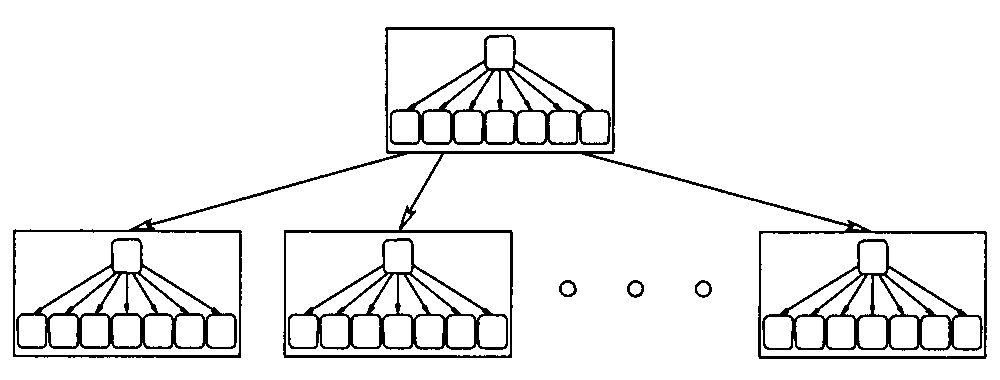
\includegraphics[width=\columnwidth]{b-tree.png}
\caption{Self-similiar \emph{tree within a tree} structure~\cite{chen2002fractal}}
\label{fig:b-tree}
\end{figure}

\subsection{Flash as Cache Extension (\subsecit{FaCE})}
FaCE~\cite{kang2012flash} utilizes flash memory as an extension to a DRAM buffer for a recoverable database. It caches data pages in flash memory on exit from the DRAM buffer, essentially resulting in a low-overhead cache hierarchy extension. Flash cache is capable of sustaining high hit rates without incurring excessive run-time overheads. In certain situations, this technique can be more cost efficient than increasing the size of DRAM buffers. It also allows a more sustainable I/O performance for higher transaction throughput. Another advantage is the minimized overhead in recovery scenarios and an accelerated system restart after failure.

\section{Current Research}
It is to be expected that classic HDDs are quickly approaching the end of their research possibilities. The research of hard disk technology is primarily focused on density increase, which is stagnating since SSDs entered the market and bit sizes are quickly approaching physical limits.
\\
SSD and in general solid state technologies are still young and provide high potential for improvements and innovations.
\\
In the following section we present two major advances in non-volatile memory technology emerging in the latest years.

\subsection{Phase Change Memory}
Phase-change memory (\emph{PRAM}) is a non-volatile type of memory which uses the unique chemical behaviour of chalcogenide glass: by applying a voltage to amorphous chalcogenide glass; heating up to the crystallization temperature for around 100 ns, the glass crystallizes. In this form the resistance over the material is much lower. By heating it to a temperature above the crystallization temperature for 50 ns and instantly letting it cool, it returns back to the amorphous state with higher resistance.
\\
Phase-Change Memory therefore does not have the need for an erase step before writing. Each cell can individually be set or reset at will. This allows for simpler controllers, not requiring many of the complex optimizations like garbage collection done in flash transaction layers, while still having the benefits of a non-mechanical state memory. Also, degradation is much lower: cells last for up to 100 million set/reset cycles, instead of 100 thousand program/erase cycles in SLC NAND flash. Also, less cycles are required because write amplification from garbage collection does not occur.
\\
However, as of 2014, PRAM has not yet been available for consumers and prices have not been competitive. In early 2014, Micron, one of the largest contributors to PRAM research, has taken all information regarding PRAM out of its portfolio --- some manufacturers like IBM still do research on PRAM technology.

\subsection{Self-healing NAND Flash Memory}
NAND flash cells become useless after many program/erase cycles because of the trapped charge, which means current SSDs do not survive in a server environment for long and must be replaced often.
\\
To extend the disk lifetime and reduce the maintaining costs, a process called self-healing through thermal annealing can be used, where trapped charge in flash cells is released by heating the chip to a high temperature ($\sim 200~^{\circ}$C) for half an hour~\cite{wu2011exploiting}. After this process, 80\% of the trapped charge is release and the cells can be re-used. This process can be applied approximately 25 times per chip, after that time, the remaining trapped charge will be too high. Overall, using thermal annealing can bring a 6$\times$ improvement in disk lifetime.
\\
Thermal annealing has two downsides: Heating consumes a lot of energy, which makes its use limited in mobile devices and might require additional cooling architecture, and it comes at a greater cost. The chips themselves need to be built so that a heater can be placed on or inside of them, making them more expensive, and there need to be backup chips holding the data while other chips are being heated, reducing the total available memory.

\section{Future Trends}
Current SSD prices are still high --- while, as of 2014, 1 TiB of enterprise SSD storage costs around \EUR{1,500} to \EUR{2,000} and a server with 1 TiB of main memory will cost from \EUR{10,000} to \EUR{15,000}, there is also a speed improvement of one order of magnitude in both access time and read/write speed. In a production environment, instead of extending the cache layer hierarchy by an SSD layer, the consideration of increasing main memory first is important, especially in cases where the working set could fit in main memory. In our opinion, maximizing main memory before investing in the necessary software to properly use SSD storage is preferable in most cases.

\section{Conclusion}
We have provided an overview of computer secondary storage, comparing hard disk drives and solid state drives and displaying the advantages and disadvantages of using SSD storage in server environments.
Following this, we discussed the various design implications and difficulties for both SSD producers and consumers.
We have presented techniques for mitigating these problems and presented two possible new techniques in the field.

\bibliographystyle{unsrt}
\bibliography{secondary-storage}
%  and remember to run:
% latex bibtex latex latex
% to resolve all references

\balancecolumns
\end{document}
